\section{Анализ существующих композиторов Wayland}
\subsection{Weston}
Weston --- это референсная реализация композитора Wayland. Weston поставляется с несколькими примерами клиентов, от простых, которые демонстрируют некоторые аспекты протокола для, до полных клиентов и упрощенного инструментария. Существует также полноценный эмулятор терминала (weston-terminal) и простая оболочка рабочего стола. Наконец, Weston также обеспечивает интеграцию с сервером Xorg и может разместить X-клиенты на рабочем столе Wayland и представляться им как ОМ X. Пример запуска Weston привежен на рисунке \ref{fig:weston}.

\begin{figure}[h!]
\center{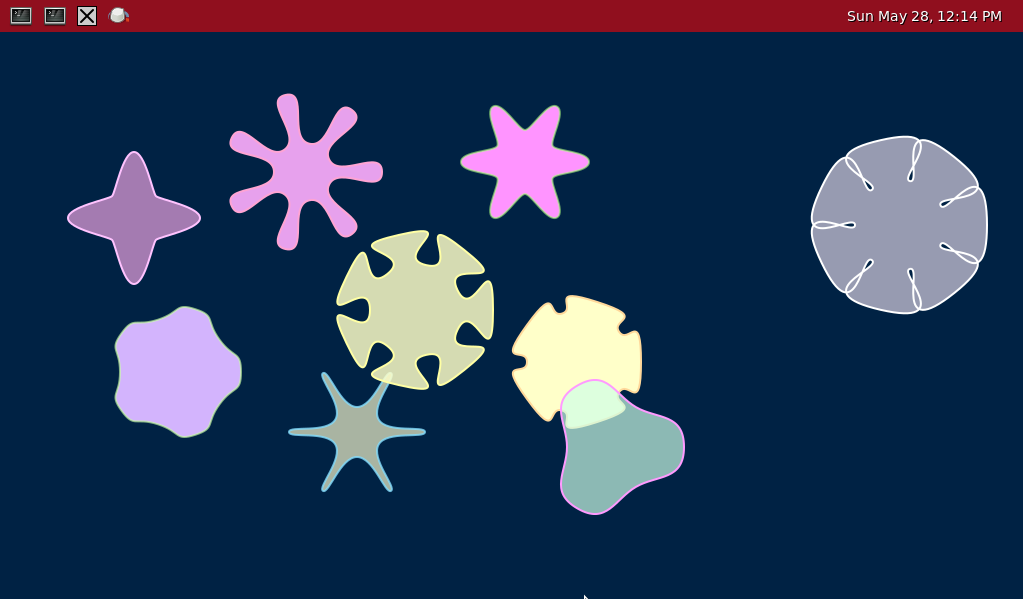
\includegraphics[width=\linewidth]{weston}}
\caption{Рабочий стол Weston}
\label{fig:weston}
\end{figure}

Weston по умолчанию поддерживает несколько бекендов, что позволяет ему без проблем запускаться на большом количестве платформ. До версии 1.9 Weston так же поддерживал бекенд для проприетарной графической системы Raspberry Pi, однако разработчики отказались от этой части из-за сложности поддержки кода.

Пакет Weston по умолчанию включает в себя библиотеку libweston. Libweston --- это попытка отделить переиспользуемый исхдный код Weston в отдельную библиотеку. Эта библиотека включает в себя корректную реализацию всех базовых протоколов Wayland и взаимодействие с подсистемами ввода вывода. Libweston предлагается использовать для облегчения разработки собственных ОМ.

Libweston впервые появился в версии Weston 1.12. В настоящее время библиотека находится в состоянии активной разработки. Разработчики утверждают, что API библиотеки не стабилен может сильно изменяться от версии к версии, поэтому в данный момент использование этой библиотеки не самое лучшее решение. 

\subsection{WLC}
WLC --- популярная библиотека-композитор для Wayland~\cite{wlc}. На основе этой библиотеки реализовано несколько оконных менеджеров и других библиотек. Их примеры:
\begin{itemize}
\item Тайлинговый оконный менеджер Sway (рис.~\ref{fig:sway})
\item Модульный композитор orbment
\item Модульный ОМ fireplace
\end{itemize}

\begin{figure}[h!]
\center{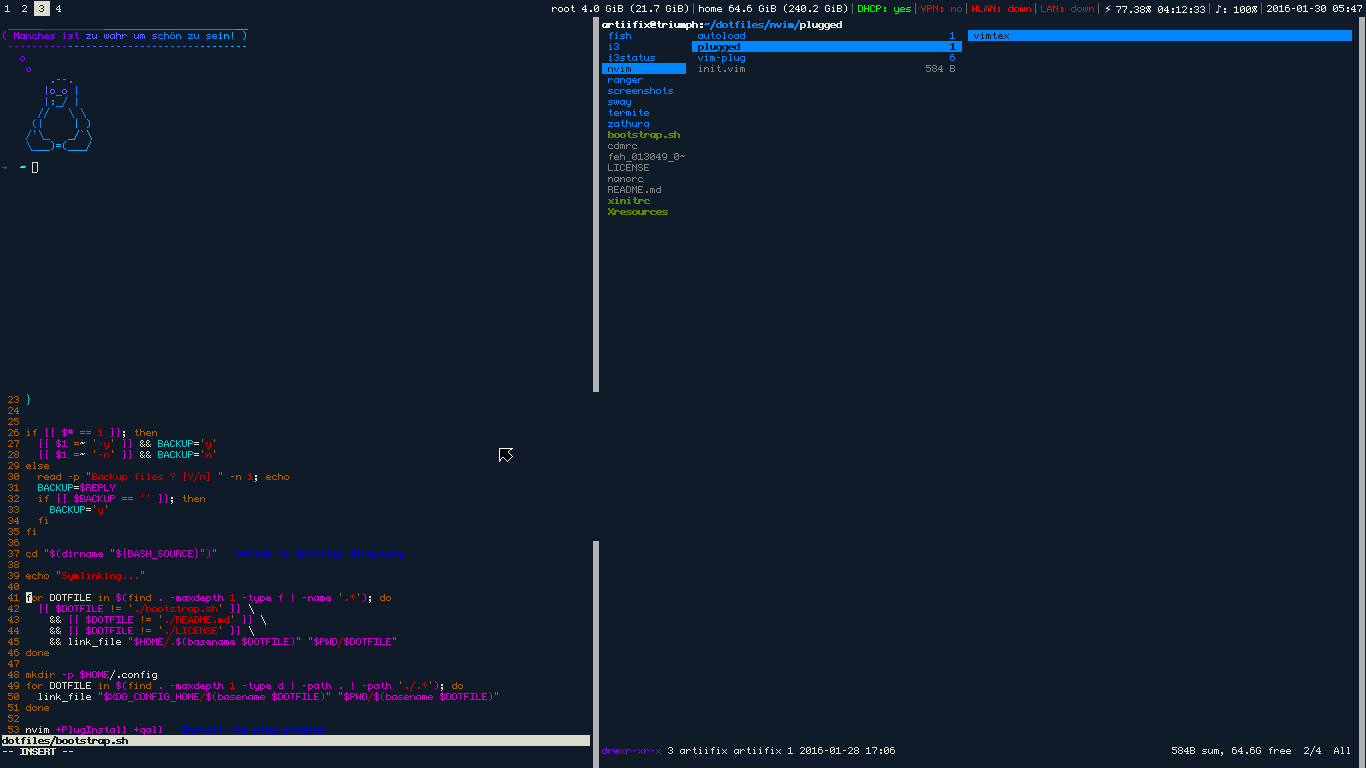
\includegraphics[width=\linewidth]{sway}}
\caption{Пример Sway}
\label{fig:sway}
\end{figure}

Библиотека обладает большой функциональностью. Она поддерживает различные бекенды, может запускаться как под X11, так и под Wayland. Библиотека очень удобна для разработки на ее основе собственного ОМ, так как она содержит примеры написания простейших ОМ.

\subsection{SWC}
SWC --- это небольшой композитор Wayland, реализованный в виде библиотеки. Разработчик SWC утверждает, что swc был написан с целью предоставить минимальный набор функций для возможности отображения окон на экране.

На основе SWC реализован простой оконный менеджер Velox, предназначение которого --- продемонстрировать возможности библиотеки.

\begin{figure}[h!]
\center{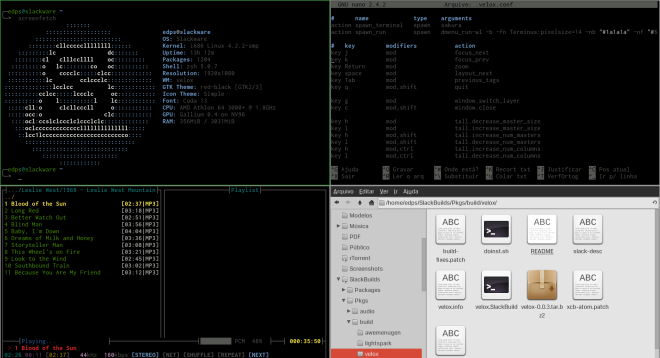
\includegraphics[width=\linewidth]{velox}}
\caption{ОМ Velox}
\label{fig:velox}
\end{figure}

